\chapter{CRISP-DM}\label{chp:crisp}

Für den Verlauf dieser Arbeit wird eine Vorgehensweise aus dem Bereich des Data Mining verwendet, da diese gute Anwendungsmöglichkeiten für Projekte im Bereich ML bietet. Diese wird \ac{CRISP-DM} genannt. Der CRISP-DM wird verwendet, um den Lebenszyklus von Daten innerhalb eines Data Mining Projekts zu modellieren und ein dafür geeignetes Data Mining-Modell zu entwickeln. Der Prozess wird dabei in sechs verschiedene Phasen unterteilt, die unterschiedliche Ziele verfolgen \parencite[vgl.][S. 1]{.Wirth}.

\begin{figure}[H]
	\centering
	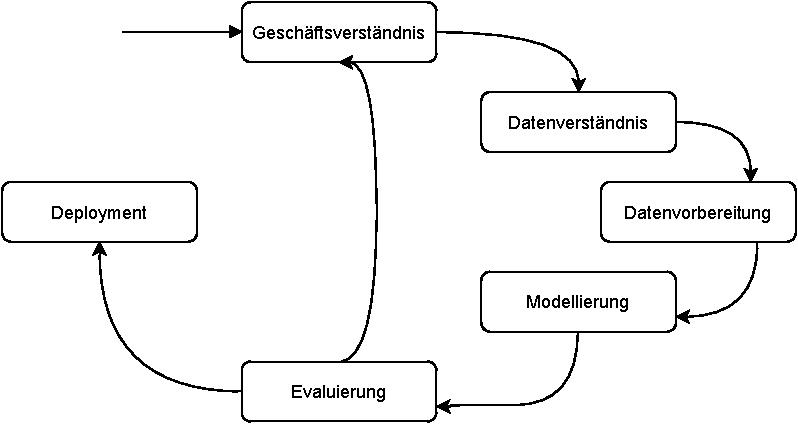
\includegraphics[scale=0.9]{images/CRISP.pdf}
	\caption{Ablauf eines CRISP-DM: Eigene Abbildung in Anlehnung an \parencite[][S. 5]{.Wirth}}
	\label{figure:ablauf-crisp-dm}
\end{figure}

In der ersten Phase geht es darum, die Ziele und die Anforderungen des Projekts zu untersuchen und diese in ein Data Mining-Problem zu übertragen. Anschließend muss sich der Entwickler mit den Daten vertraut machen. Dazu gehört beispielsweise das Gewährleisten der Datenqualität oder Erkenntnisse über die Daten, wie zum Beispiel deren Ursprung, zu sammeln. Nachdem die Daten untersucht wurden, werden diese so vorbereitet, dass sie in das ML-Modell eingefügt und mit ihnen gearbeitet werden kann. Dazu gehört unter anderem, doppelt vorkommende Datensätze oder Ausreißer zu entfernen. Anschließend kann damit begonnen werden, das Modell zu erstellen und die Ergebnisse zu evaluieren. Stellt sich nach der Evaluation heraus, dass nicht alle Anforderungen an das Modell erfüllt wurden, wird erneut damit begonnen, die Anforderungen zu definieren und die Daten zu analysieren, vorzubereiten und ein neues Modell zu erstellen. Erst nachdem alle Anforderungen erfüllt wurden, kann das Modell für den produktiven Gebrauch verwendet werden \parencite[vgl.][S. 5ff.]{.Wirth}.

% An diesen Phasen wird sich der Aufbau dieser Arbeit orientieren. In \vref{chp:problemanalyse-und-datenvorbereitung} wird damit begonnen, das vorliegende Problem zu analysieren und die Daten vorzubereiten. Anschließend werden in \vref{chp:entwicklung-verschiedener-loesungsansaetze} mögliche Modelle und Lösungsansätze entwickelt und in \vref{chp:evaluierung-2} analysiert und evaluiert. Da der Fokus dieser Arbeit auf der Erörterung der Sinnhaftigkeit von Anwendungen von Filtertechniken liegt, wird die Phase des Deployments nicht beachtet und ausgelassen. Auch eine erneute Analyse des Datenverständnisses wird in dieser Arbeit nicht thematisiert. Die Modellierung entspricht dabei der Entwicklung verschiedener Filtertechniken.